\documentclass[12pt,a4paper]{article}
\usepackage[utf8]{inputenc}
\usepackage[turkish]{babel}
\usepackage{amsmath,amssymb,amsfonts,amsthm}
\usepackage{geometry}
\geometry{top=2.5cm,bottom=2.5cm,left=2.5cm,right=2.5cm}
\usepackage{xcolor}
\usepackage{tikz}
\usetikzlibrary{babel,arrows.meta,positioning,calc}
\usepackage{pgfplots}
\pgfplotsset{compat=1.18}
\usepackage[most]{tcolorbox}
\usepackage{hyperref}
\usepackage{caption}
\usepackage{booktabs}
\usepackage{tabularx}

% -------------------------------------------------
% style.tex – Ortak paketler ve tcolorbox tanımları
% -------------------------------------------------
\usepackage[utf8]{inputenc}
\usepackage[turkish]{babel}
\usepackage{amsmath,amssymb,amsfonts,amsthm}
\usepackage{geometry}
\geometry{top=2.5cm,bottom=2.5cm,left=2.5cm,right=2.5cm}
\usepackage{xcolor}
\usepackage{tikz,pgfplots}
\pgfplotsset{compat=1.18}
\usepackage[most]{tcolorbox}
\usepackage{hyperref}
\usepackage{caption,booktabs,tabularx}

% ---------- Renk tanımları ----------
\definecolor{purp}{RGB}{102,51,153}
\definecolor{tealblue}{RGB}{0,120,130}
\definecolor{mainblue}{RGB}{26,82,118}
\definecolor{alertred}{RGB}{180,40,40}
\definecolor{okgreen}{RGB}{34,139,34}

% ---------- Tek‑argümanlı kutular ----------
\newtcolorbox{box}[2][]{
  colback=white,
  colframe=purp,
  title={#2},
  arc=2mm,
  breakable,
  #1
}

\newtcolorbox{uyari}[1][]{
  colback=yellow!10,
  colframe=orange,
  title={Uyarı},
  arc=2mm,
  breakable,
  #1
}

% ---------- Diğer yardımcı kutular (isteğe bağlı) ----------
\newtcolorbox{ornek}[2][]{
  colback=mainblue!5!white,
  colframe=mainblue,
  title={#2},
  arc=2mm,
  breakable,
  #1
}

\newtcolorbox{odev}[2][]{
  colback=okgreen!5!white,
  colframe=okgreen,
  title={Çözümü Olmayan Ödev ve Tam Çözümü: #2},
  arc=2mm,
  breakable,
  #1
}

\newtcolorbox{tanim}[2][]{
  colback=gray!5!white,
  colframe=gray!60!black,
  title={#2},
  arc=2mm,
  breakable,
  #1
}

\newtcolorbox{sezgi}[2][]{
  colback=tealblue!5!white,
  colframe=tealblue,
  title={Sezgisel Bakış ve Basit Anlatım: #2},
  arc=2mm,
  breakable,
  #1
}


\title{\textbf{İSTATİSTİK TEORİSİ}\\[0.3em] \Large 6. Hafta Ders Notları: En Çok Olabilirlik (MLE) ve Rao-Cramér Sınırı}
\author{Ders Notları Düzenlemesi, Sezgisel Açıklamalar ve Çözümlü Analizler}
\date{}

\begin{document}
\maketitle

\begin{abstract}
Bu çalışma; İstatistik Teorisi dersinin 6. haftasında yer alan \textbf{Olabilirlik İlkesi}, \textbf{En Çok Olabilirlik Tahmini (MLE)}, \textbf{Zehna Değişmezlik Teoremi}, \textbf{Skor Fonksiyonu}, \textbf{Fisher Bilgisi} ve \textbf{Rao-Cramér Alt Sınırı (CRLB / UMVUE)} konularını içermektedir. Nokta tahmininin bu en kritik araçları sezgisel benzetmeler ve tam çözümlü örneklerle ele alınmıştır.
\end{abstract}

\hrule
\vspace{1em}

\section{Büyük Resim: 6. Haftada Ne Öğreniyoruz ve Neden?}

\begin{sezgi}{Nokta Tahmini ve Sherlock Holmes Mantığı (MLE)}
Olasılık teorisinde kitle parametresi ($\theta$) bilinir ve *"elimdeki torbadan kırmızı bilye gelme olasılığı nedir?"* sorusu sorulur.  
İstatistik teorisinde ise durum tam tersidir: **Torbanın içini bilmiyoruz!**  
Elimizde sadece torbadan çekilmiş bir örneklem ($x_1, x_2, \dots, x_n$) vardır.  
Soru şudur: *"Mevcut veriyi üretmiş olma ihtimali en yüksek olan $\theta$ parametresi hangisidir?"*  
İşte bu soruya cevap veren yöntem \textbf{En Çok Olabilirlik Yöntemi (MLE)}'dir.  
Peki bulduğumuz tahmin edicinin "en iyisi" olduğunu nereden biliriz? Evrende yapılabilecek en kusursuz tahminin varyansı için konulmuş bir fiziksel alt sınır vardır; buna da **Rao-Cramér Alt Sınırı (CRLB)** denir.
\end{sezgi}

---

\section{Olabilirlik ve En Çok Olabilirlik Yöntemi (MLE)}

\begin{tanim}{Olabilirlik ve Log-Olabilirlik Fonksiyonu}
$X_1, X_2, \dots, X_n \overset{\text{i.i.d.}}{\sim} f_\theta(x)$ olsun. Örneklem verisi $x_1, \dots, x_n$ toplandıktan sonra, parametre $\theta$'nın \textbf{Olabilirlik Fonksiyonu}:
\begin{equation}
    L(\theta) = L(\theta; x_1, \dots, x_n) = \prod_{i=1}^n f_\theta(x_i)
\end{equation}
ve çarpımları toplama çevirerek türev almayı kolaylaştıran \textbf{Log-Olabilirlik Fonksiyonu}:
\begin{equation}
    \ell(\theta) = \ln L(\theta) = \sum_{i=1}^n \ln f_\theta(x_i)
\end{equation}
şeklinde tanımlanır.
\end{tanim}

\begin{tanim}{En Çok Olabilirlik Tahmin Edicisi (MLE)}
Gözlenen veriyi üretme olasılığını (olabilirliğini) maksimize eden parametre değeri $\hat{\theta}_{\text{MLE}}$'dir:
\begin{equation}
    \hat{\theta}_{\text{MLE}} = \arg\max_{\theta \in \Theta} L(\theta) = \arg\max_{\theta \in \Theta} \ell(\theta)
\end{equation}
$\ell(\theta)$ fonksiyonu içbükey (konkav) ve türevlenebilir ise en çok olabilirlik denklemi (skor denklemi):
\begin{equation}
    \frac{d\ell(\theta)}{d\theta} = 0
\end{equation}
ve tepe noktasını doğrulamak için ikinci mertebe koşulu $\left. \frac{d^2\ell(\theta)}{d\theta^2} \right|_{\theta = \hat{\theta}} < 0$'dır.
\end{tanim}

\begin{center}
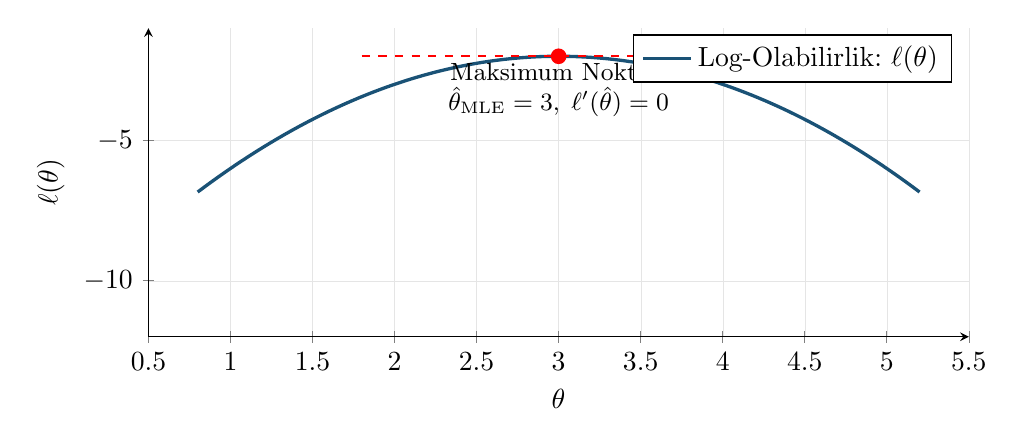
\begin{tikzpicture}
\begin{axis}[
    width=12cm, height=5.5cm,
    axis lines=left,
    xlabel={$\theta$}, ylabel={$\ell(\theta)$},
    xmin=0.5, xmax=5.5, ymin=-12, ymax=-1,
    samples=100, domain=0.8:5.2,
    grid=both, grid style={line width=.1pt, draw=gray!20}
]
    \addplot[mainblue, very thick] {- (x - 3)^2 - 2};
    \addlegendentry{Log-Olabilirlik: $\ell(\theta)$}

    \draw[dashed, red, thick] (axis cs:1.8, -2) -- (axis cs:4.2, -2);
    \node[circle, fill=red, inner sep=2pt] at (axis cs:3, -2) {};
    \node at (axis cs:3, -3.2) [font=\small, align=center] {Maksimum Noktası\\$\hat{\theta}_{\text{MLE}} = 3, \; \ell'(\hat{\theta}) = 0$};
\end{axis}
\end{tikzpicture}
\captionof{figure}{Log-olabilirlik fonksiyonu ve tepe noktasında eğimin sıfır olduğu ($\ell'(\theta)=0$) MLE çözümü.}
\end{center}

\begin{ornek}{Örnek 1: $N(\theta, 1)$ Dağılımında $\theta$'nın MLE'si}
$f(x_i) = \frac{1}{\sqrt{2\pi}} e^{-\frac{1}{2}(x_i - \theta)^2}$.
\begin{equation}
    \ell(\theta) = -\frac{n}{2} \ln(2\pi) - \frac{1}{2} \sum_{i=1}^n (x_i - \theta)^2
\end{equation}
Türevi sıfıra eşitleyelim:
\begin{equation}
    \frac{d\ell(\theta)}{d\theta} = \sum_{i=1}^n (x_i - \theta) = 0 \implies \sum_{i=1}^n x_i - n\theta = 0 \implies \boxed{\hat{\theta}_{\text{MLE}} = \bar{X}_n}
\end{equation}
İkinci türev $\frac{d^2\ell}{d\theta^2} = -n < 0$ olduğundan yerel ve mutlak tepe noktasıdır.
\end{ornek}

\begin{ornek}{Örnek 2: $\text{Bernoulli}(p)$ Dağılımında $p$'nin MLE'si}
$P(X=x) = p^x (1-p)^{1-x}, \; x \in \{0, 1\}$. Başarı sayısı $Y = \sum_{i=1}^n X_i$ olsun:
\begin{equation}
    L(p) = p^Y (1-p)^{n-Y} \implies \ell(p) = Y \ln(p) + (n-Y) \ln(1-p)
\end{equation}
Türev:
\begin{equation}
    \frac{d\ell(p)}{dp} = \frac{Y}{p} - \frac{n-Y}{1-p} = 0 \implies Y(1-p) = p(n-Y) \implies Y = np \implies \boxed{\hat{p}_{\text{MLE}} = \frac{Y}{n} = \bar{X}_n}
\end{equation}
\end{ornek}

---

\section{MLE'nin Temel Özellikleri}

\subsection{1. Değişmezlik Özelliği (Invariance Property - Zehna Teoremi)}

\begin{tanim}{Zehna Teoremi}
Eğer $\hat{\theta}$, $\theta$ parametresinin en çok olabilirlik tahmin edicisi ise, herhangi bir $g(\theta)$ fonksiyonunun en çok olabilirlik tahmin edicisi de doğrudan:
\begin{equation}
    \boxed{\widehat{g(\theta)}_{\text{MLE}} = g(\hat{\theta}_{\text{MLE}})}
\end{equation}
olur.
\end{tanim}

\begin{sezgi}{Zehna Teoreminin Muazzam Pratikliği}
Yansız tahmin ediciler fonksiyon dönüşümlerinde bozulur: $\hat{\theta}$ yansız olsa bile $g(\hat{\theta})$ genellikle $g(\theta)$ için yansız \textbf{değildir} ($E[g(\hat{\theta})] \neq g(E[\hat{\theta}])$).  
Fakat MLE'de böyle bir dert yoktur! Örneğin $\lambda$'nın MLE'si $\bar{X}$ ise; $\lambda^2$'nin MLE'si doğrudan $\bar{X}^2$, $e^{-\lambda}$'nın MLE'si ise doğrudan $e^{-\bar{X}}$ olur.
\end{sezgi}

\begin{odev}{Poisson Sürecinde Boş Bırakılan Problem ve Çözümü}
\textbf{Soru (Sayfa 39):} $X_1, \dots, X_n \overset{\text{i.i.d.}}{\sim} \text{Poisson}(\lambda)$ olsun. $\eta = g(\lambda) = e^{-2\lambda}$ parametresinin en çok olabilirlik tahmin edicisini bulunuz ve yansızlığını inceleyiniz. *(Notlarda soru sorulup çözümü boş bırakılmıştır).*

\bigskip
\textbf{Detaylı Çözüm Adımları:}
\begin{enumerate}
    \item Önce ana parametre $\lambda$'nın MLE'sini bulalım:
    \begin{align}
        L(\lambda) &= \frac{e^{-n\lambda} \lambda^{\sum x_i}}{\prod x_i!} \implies \ell(\lambda) = -n\lambda + \left(\sum_{i=1}^n x_i\right) \ln\lambda - \ln\left(\prod x_i!\right) \notag \\
        \frac{d\ell(\lambda)}{d\lambda} &= -n + \frac{\sum x_i}{\lambda} = 0 \implies \hat{\lambda}_{\text{MLE}} = \bar{X}_n
    \end{align}
    \item Zehna değişmezlik özelliği gereğince $\eta = e^{-2\lambda}$'nın MLE'si:
    \begin{equation}
        \boxed{\hat{\eta}_{\text{MLE}} = e^{-2\hat{\lambda}} = e^{-2\bar{X}_n}}
    \end{equation}
    \item \textbf{Yansızlık İncelemesi:}  
    Beklenen değerini hesaplayalım ($Y = \sum X_i \sim \text{Poisson}(n\lambda)$):
    \begin{align}
        E(\hat{\eta}) &= E\left( e^{-\frac{2}{n}\sum_{i=1}^n X_i} \right) = \left[ M_X\left(-\frac{2}{n}\right) \right]^n = \left[ e^{\lambda(e^{-2/n} - 1)} \right]^n = \exp\left( n\lambda(e^{-2/n} - 1) \right)
    \end{align}
    $n(e^{-2/n} - 1) \neq -2$ olduğundan sonlu örneklemde $\hat{\eta}$ \textbf{yansız değildir}.  
    Ancak $n \to \infty$ iken Taylor açılımından $n(e^{-2/n} - 1) \to -2$ olur:
    \begin{equation}
        \lim_{n \to \infty} E(\hat{\eta}) = e^{-2\lambda} = \eta
    \end{equation}
    Yani tahmin edici \textbf{asemptotik olarak yansız ve tutarlıdır}.
\end{enumerate}
\end{odev}

---

\section{Fisher Bilgisi ve Rao-Cramér Eşitsizliği (CRLB)}

\begin{tanim}{Skor Fonksiyonu ve Fisher Bilgisi}
Tek bir gözlem $X \sim f_\theta(x)$ için \textbf{Skor Fonksiyonu}:
\begin{equation}
    U_\theta(X) = \frac{d}{d\theta} \ln f_\theta(X)
\end{equation}
Regülerlik koşulları altında skor fonksiyonunun beklenen değeri sıfırdır:
\begin{equation}
    E_\theta[U_\theta(X)] = 0
\end{equation}
\textbf{Fisher Bilgisi (Fisher Information)}, bu skor fonksiyonunun varyansıdır:
\begin{equation}
    \boxed{I(\theta) = V_\theta(U_\theta(X)) = E_\theta\left[ \left( \frac{d}{d\theta} \ln f_\theta(X) \right)^2 \right] = - E_\theta\left[ \frac{d^2}{d\theta^2} \ln f_\theta(X) \right]}
\end{equation}
$n$ boyutlu bağımsız örneklem için toplam bilgi: $I_n(\theta) = n I(\theta)$'dır.
\end{tanim}

\begin{sezgi}{Fisher Bilgisinin Geometrik ve Sezgisel Anlamı}
İkinci türev $-\frac{d^2 \ell}{d\theta^2}$ log-olabilirlik eğrisinin tepe noktasındaki **eğriliğini (kavisini)** ölçer:
\begin{itemize}
    \item Eğer tepe çok sivri ve dik ise: Eğrilik büyüktür $\implies$ Fisher Bilgisi büyüktür. Bu demektir ki veriler doğru parametreyi nokta atışı işaret eder; tahmin hatası ve varyansı küçüktür!
    \item Eğer tepe yayvan ve düz ise: Eğrilik küçüktür $\implies$ Fisher Bilgisi azdır. Veriler parametre hakkında yetersiz bilgi taşır.
\end{itemize}
\end{sezgi}

\begin{tanim}{Rao - Cramér Alt Sınırı (CRLB)}
$T_n = T(X_1, \dots, X_n)$ yansız bir tahmin edici ($E_\theta(T_n) = \theta$) ise, varyansı hiçbir zaman belirli bir sınırın altına inemez:
\begin{equation}
    \boxed{V_\theta(T_n) \ge \frac{1}{n I(\theta)} = \text{CRLB}}
\end{equation}
Eğer yansız bir tahmin edicinin varyansı bu sınıra eşit çıkarsa ($V(T_n) = \text{CRLB}$), o tahmin ediciye \textbf{En Küçük Varyanslı Düzgün Yansız Tahmin Edici (UMVUE / MVUE)} veya \textbf{Tam Etkin (Efficient)} tahmin edici denir.
\end{tanim}

\begin{uyari}
\textbf{Notlardaki Sembolik Düzeltme (Sayfa 42):}
Notta Poisson örneği çözülürken parametre için hem $\theta$ hem $\lambda$ sembolleri birbirinin yerine kullanılmıştır. Standart kitle parametresi olarak $\lambda$ alınmıştır.
\end{uyari}

\begin{ornek}{Örnek 3: $\text{Poisson}(\lambda)$ Dağılımında CRLB ve UMVUE}
$f(x) = \frac{e^{-\lambda}\lambda^x}{x!}$ dağılımı için:
\begin{align}
    \ln f(x) &= -\lambda + x \ln\lambda - \ln(x!) \\
    \frac{d}{d\lambda} \ln f(x) &= -1 + \frac{x}{\lambda} \\
    \frac{d^2}{d\lambda^2} \ln f(x) &= -\frac{x}{\lambda^2}
\end{align}
Tek gözlemin Fisher bilgisi:
\begin{equation}
    I(\lambda) = -E\left( -\frac{X}{\lambda^2} \right) = \frac{E(X)}{\lambda^2} = \frac{\lambda}{\lambda^2} = \frac{1}{\lambda}
\end{equation}
$n$ boyutlu örneklem için Rao-Cramer Alt Sınırı:
\begin{equation}
    \text{CRLB} = \frac{1}{n I(\lambda)} = \frac{1}{n (1/\lambda)} = \frac{\lambda}{n}
\end{equation}
Şimdi örneklem ortalaması $\bar{X}_n$'in varyansına bakalım:
\begin{equation}
    V(\bar{X}_n) = \frac{V(X)}{n} = \frac{\lambda}{n}
\end{equation}
Görüldüğü üzere $V(\bar{X}_n) = \text{CRLB} = \frac{\lambda}{n}$'dir.  
Dolayısıyla $\bar{X}_n$, $\lambda$ parametresi için \textbf{UMVUE}'dir (daha düşük varyanslı bir yansız tahmin edici bulmak matematiksel olarak imkansızdır!).
\end{ornek}

\begin{center}
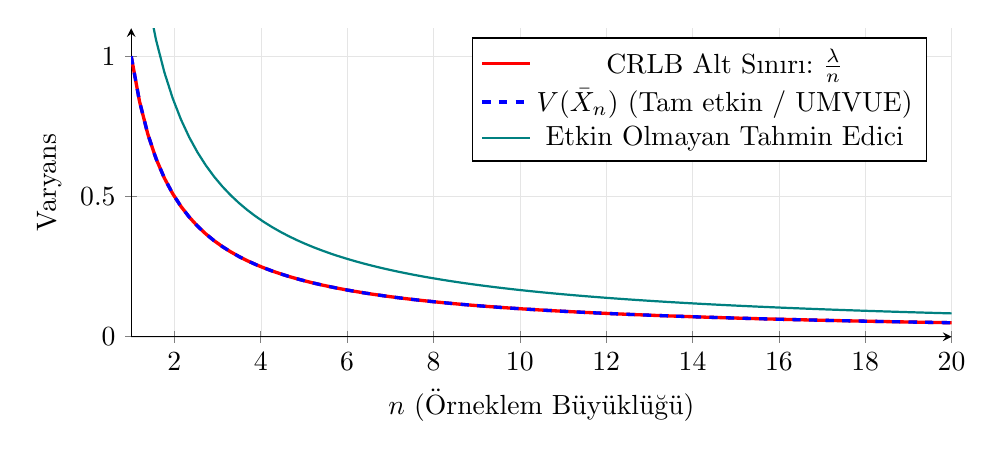
\begin{tikzpicture}
\begin{axis}[
    width=12cm, height=5.5cm,
    axis lines=left,
    xlabel={$n$ (Örneklem Büyüklüğü)}, ylabel={Varyans},
    xmin=1, xmax=20, ymin=0, ymax=1.1,
    samples=100, domain=1:20,
    legend pos=north east,
    grid=both, grid style={line width=.1pt, draw=gray!20}
]
    \addplot[red, very thick] {1 / x};
    \addlegendentry{CRLB Alt Sınırı: $\frac{\lambda}{n}$}

    \addplot[blue, dashed, very thick] {1 / x};
    \addlegendentry{$V(\bar{X}_n)$ (Tam etkin / UMVUE)}

    \addplot[teal, thick] {1 / (0.6 * x)};
    \addlegendentry{Etkin Olmayan Tahmin Edici}
\end{axis}
\end{tikzpicture}
\captionof{figure}{Örneklem büyüklüğü arttıkça Rao-Cramer alt sınırının azalması ve UMVUE varyansının bu sınıra tam oturması.}
\end{center}

---

\section{6. Hafta Hızlı Tekrar ve Karşılaştırma Tablosu}

\begin{table}[ht]
\centering
\small
\renewcommand{\arraystretch}{1.35}
\begin{tabularx}{\textwidth}{@{}l l X@{}}
\toprule
\textbf{Kavram} & \textbf{Matematiksel Formül} & \textbf{Ne İşe Yarar / Sezgisel Anlamı} \\ \midrule
\textbf{Olabilirlik $L(\theta)$} & $\prod_{i=1}^n f(x_i; \theta)$ & Verilen verinin gerçekleşme ihtimalini parametrenin fonksiyonu yapar. \\
\textbf{MLE ($\hat{\theta}$)} & $\arg\max \ell(\theta) \implies \ell'(\theta) = 0$ & Veriyi en olası kılan parametre değerini bulur. \\
\textbf{Zehna Teoremi} & $\widehat{g(\theta)}_{\text{MLE}} = g(\hat{\theta}_{\text{MLE}})$ & Parametre tahmini biliniyorsa fonksiyonunun tahmini doğrudan yerine koymadır. \\
\textbf{Skor Fonksiyonu} & $U(\theta) = \frac{d}{d\theta}\ln f(X)$ & Log-olabilirliğin eğimidir; beklenen değeri daima sıfırdır ($E(U)=0$). \\
\textbf{Fisher Bilgisi} & $I(\theta) = -E[\ell''(\theta)]$ & Log-olabilirliğin tepe sivrilğidir; parametre hakkındaki bilgi miktarını ölçer. \\
\textbf{CRLB} & $\text{Alt Sınır} = \frac{1}{n I(\theta)}$ & Yansız bir tahmin edicinin sahip olabileceği teorik minimum varyanstır. \\
\textbf{UMVUE} & $V(\hat{\theta}) = \text{CRLB}$ & Alt sınıra ulaşan, en küçük varyanslı kusursuz yansız tahmin edici. \\ \bottomrule
\end{tabularx}
\caption{6. Haftanın Temel Olabilirlik ve Optimal Tahmin Kavramları Özeti}
\end{table}

\end{document}
